\section{Dagster}
Deze Proof of Concept zal gebruik maken van Dagster en MLFlow
\subsection{Installatie}
De installatie van Dagster verloopt via de package manager \texttt{pip}. Dagster ondersteunt Python versies 3.8 tot 3.12 en kan met het volgende commando worden geïnstalleerd:
\begin{minted}[frame=lines,breaklines,linenos]{bash}
    pip install dagster dagster-webserver
\end{minted}
Om Dagster te installeren op een Mac met een Apple Silicon chip moet het volgende commando gebruikt worden:
\begin{minted}[frame=lines,breaklines,linenos]{bash}
    pip install dagster dagster-webserver --find-links=https://github.com/dagster-io/build-grpcio/wiki/Wheels
\end{minted}
Na het installeren van Dagster kan er een project aangemaakt worden via de terminal met het volgende commando:
\begin{minted}[frame=lines,breaklines,linenos]{bash}
    dagster project scaffold --name my-dagster-project
\end{minted}
Het bovenstaande commando maakt een mapstructuur aan met ruimte voor de pipeline en andere bestanden voor het opzetten van een project in Dagster. Er is ook een parameter \textit{name} die de naam van het project definieert.
Na het aanmaken van het project kan de webserver worden opgestart. Dit kan met het volgende commando. Voordat je het commando uitvoert, moet je echter naar de map navigeren waar het Dagster-project zich bevindt:
\begin{minted}[frame=lines,breaklines,linenos]{bash}
    dagster dev
\end{minted}
\subsection{Dashboard}
Na het opstarten van de webserver kun je via het webadres in de terminal naar het Dagster-dashboard gaan. Het Dagster-dashboard is een omgeving waarin alle pipelines worden beheerd.
Het dashboard ziet eruit zoals in figuur~\ref{fig:Dagser_assets}
\begin{figure}
    \centering
    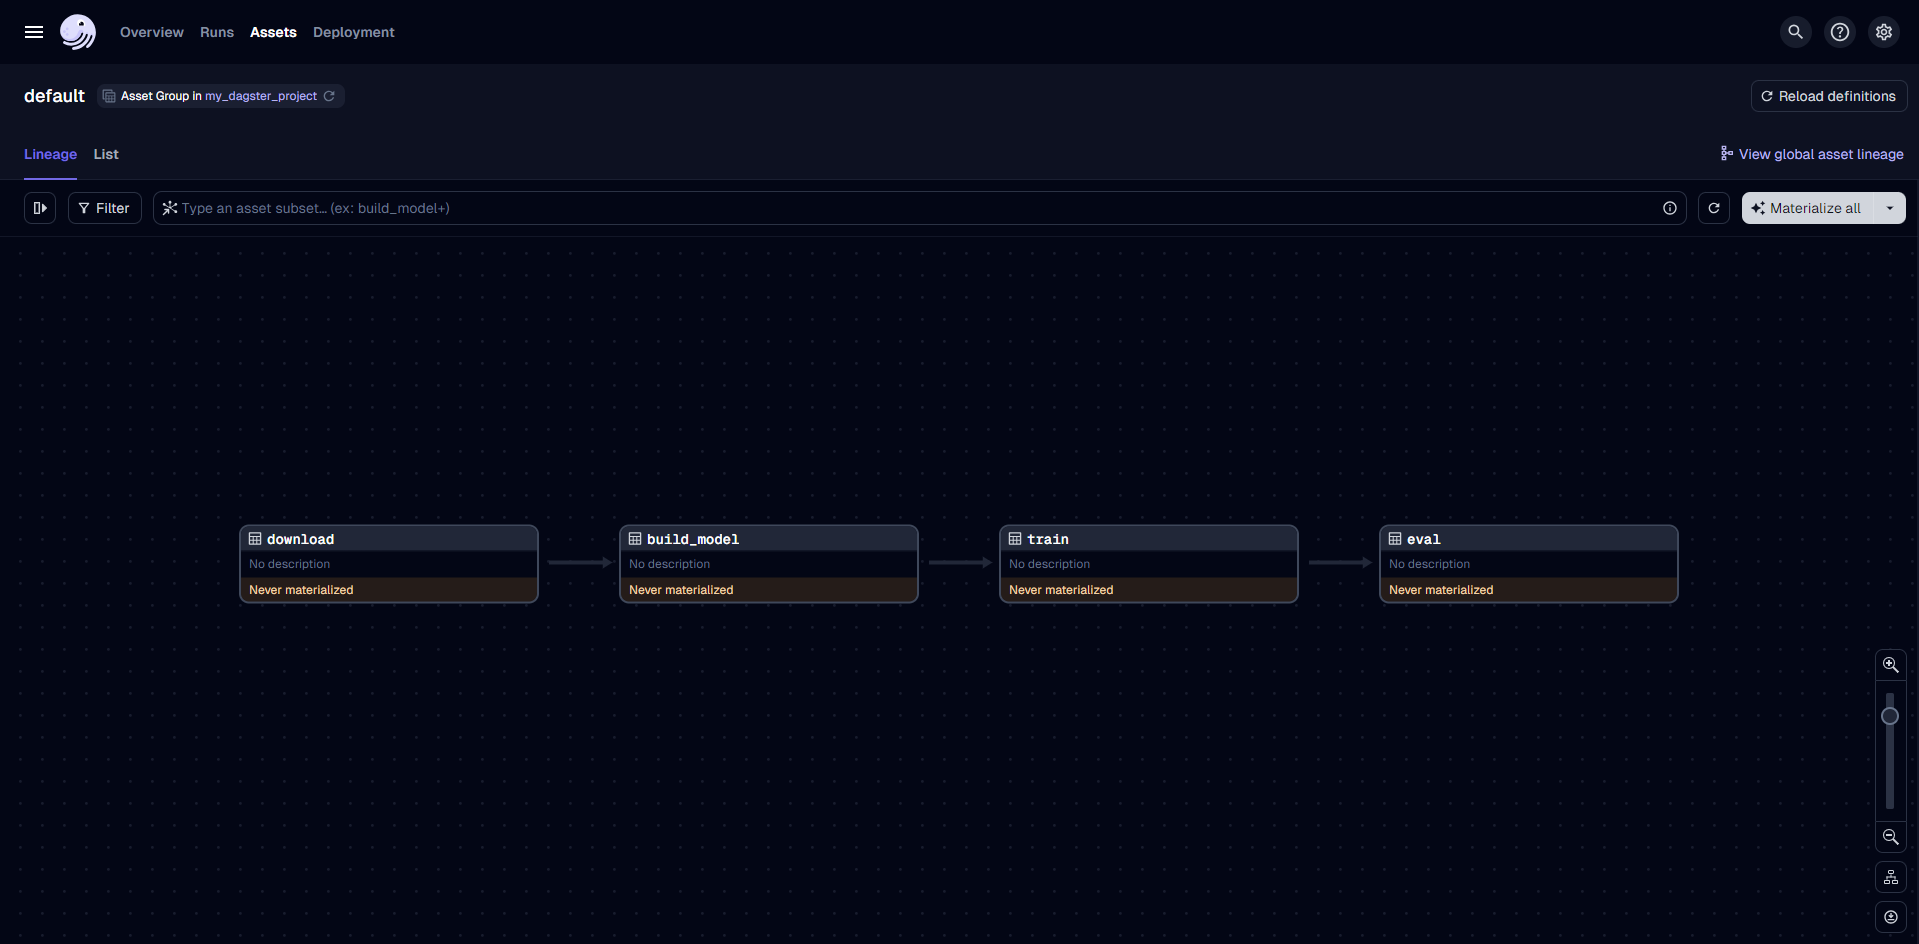
\includegraphics[width=0.9\linewidth]{graphics/Dagster_Assets.PNG}
    \caption{Dagster assets overview}
    \label{fig:Dagser_assets}
\end{figure}
Standaard wordt je naar de asset pagina van Dagster verwijst als je op de link de terminal klikt zoals in figuur~\ref{fig:Dagser_assets}
\subsection{Uitvoering}

\subsection{Pipeline}
\subsection{Problemen}
Tijdens het uitvoeren van de Proof of Concept zijn er enkele problemen opgedoken.
Het eerste probleem was dat Dagster verschillende data types niet ondersteund als parameters voor \textit{assets} waardoor het model niet meegegeven kon worden naar de opeenvolgende functie. Om dit op te lossen is het model lokaal opgeslagen om in de opeenvogende functie deze terug in te lezen en dit voor elke opeenvolgende functie.
\subsection{Cloud}